%
% $RCSfile: conditional_execution.tex,v $
%
% Copyright (c) 2002-2007. Christian Heller. All rights reserved.
%
% Permission is granted to copy, distribute and/or modify this document
% under the terms of the GNU Free Documentation License, Version 1.1 or
% any later version published by the Free Software Foundation; with no
% Invariant Sections, with no Front-Cover Texts and with no Back-Cover
% Texts. A copy of the license is included in the section entitled
% "GNU Free Documentation License".
%
% http://www.cybop.net
% - Cybernetics Oriented Programming -
%
% Version: $Revision: 1.1 $ $Date: 2007-08-01 13:59:00 $ $Author: christian $
% Authors: Christian Heller <christian.heller@tuxtax.de>
%

\subsection{Conditional Execution}
\label{conditional_execution_heading}
\index{Conditional Execution Example}

An obviously presupposed part in the previous example is a logic setting the
break \emph{condition} (flag). If the break flag was not set, the loop would
run endlessly. The following knowledge template therefore shows a
\emph{comparison} operation, as it could stand at the end of the loop's logic
model, referenced by the \emph{model} property in the previous example. After
having compared the current loop index with a maximum loop count number, the
break flag may or may not be set. When entering its next cycle, the loop
operation checks whether the flag is set. If so, the loop is stopped:

\begin{scriptsize}
    \begin{verbatim}
<model>
    <part name="comparison" channel="inline" abstraction="operation" model="compare">
        <property name="operator" channel="inline" abstraction="character" model="greater_or_equal"/>
        <property name="left_side" channel="inline" abstraction="knowledge" model=".domain.index"/>
        <property name="right_side" channel="inline" abstraction="knowledge" model=".domain.count"/>
        <property name="result" channel="inline" abstraction="knowledge" model=".domain.flag"/>
    </part>
</model>
    \end{verbatim}
\end{scriptsize}

\begin{figure}[ht]
    \begin{center}
        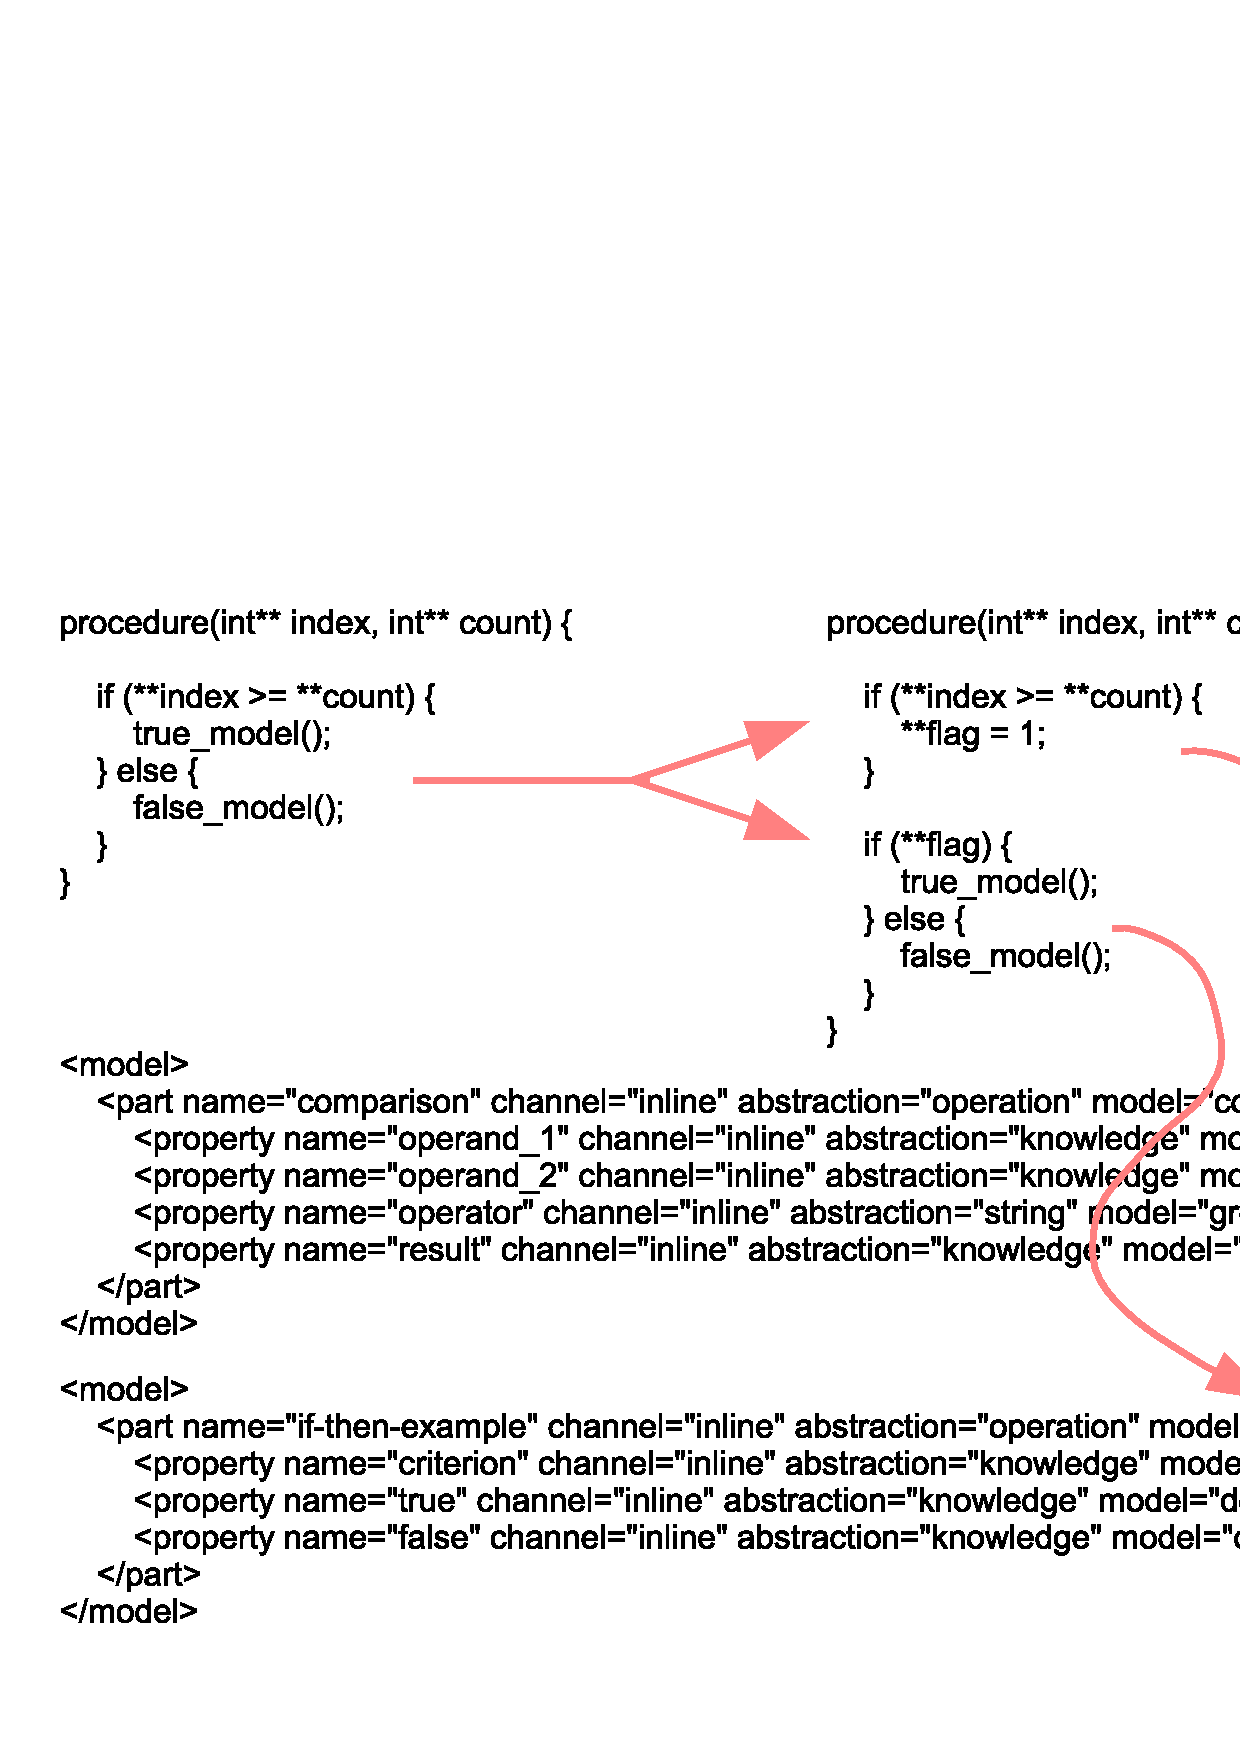
\includegraphics[scale=0.3,angle=-90]{graphics/cybolcondition.pdf}
        \caption{Condition Control Structure and Elements in C and CYBOL}
        \label{cybolcondition_figure}
    \end{center}
\end{figure}

Flags as one of the earliest techniques used in computing (in software as well
as in hardware) are the perfect means for controlling the execution of
primitive logic models, namely operations. They represent a condition set as
result of another logic model -- the latter often being some kind of comparison
operation. In order to execute code upon activation of a flag, a conventional
comparison control structure needs to be split up into two independent blocks
(figure \ref{cybolcondition_figure}), with the flag being the linking element.
The flag which was set by a comparison operation is used for branching the
control flow.

The second example shows how a classical \emph{if-then} statement would be
written in CYBOL. The corresponding operation is called \emph{branch} and it
expects three properties: a \emph{criterion} flag and two models, of which one
is executed in case the flag is \emph{true} and the other is executed otherwise.

\begin{scriptsize}
    \begin{verbatim}
<model>
    <part name="if-then-example" channel="inline" abstraction="operation" model="branch">
        <property name="criterion" channel="inline" abstraction="knowledge" model=".domain.flag"/>
        <property name="true" channel="inline" abstraction="knowledge" model=".domain.true_model"/>
        <property name="false" channel="inline" abstraction="knowledge" model=".domain.false_model"/>
    </part>
</model>
    \end{verbatim}
\end{scriptsize}
